\chapter{Simplificación de GLC}

En una GLC podemos identificar tres defectos que debemos eliminar.
\begin{enumerate}
\item Los factores comunes izquierdos.
\item La recursividad por la izquierda.
\item La ambigüedad.
\end{enumerate}

\section{Factores Comunes Izquierdos}
Una GLC tiene factores comunes izquierdos si hay por lo menos 2 producciones con el mismo símbolo en la parte izquierda y puede tener algunos símbolos coincidentes en la parte derecha.

Se tendrá formalmente:
\begin{align*}
A::=\delta\alpha_1|\delta\alpha_2|...|\delta\alpha_n|\beta_1|...|\beta_n	\quad n\geq 2, |\delta|>0
\end{align*}
Para eliminar los FCI realice la siguiente sustitución. Agregar una variable $C$ de modo que: 
\begin{align*}
&A::=\delta C|\beta_1|...|\beta_m	\\
&C::=\alpha_1|...|\alpha_n
\end{align*}

\section{La recursividad por la Izquierda}
Un símbolo no terminal $A$ es denominado recursivo por la izquierda si:
\begin{align*}
A::=Aw\qquad w\in\Sigma^*
\end{align*}
\textbf{Eliminación de Recursividad Izquierda.}\\

Las reglas de un símbolo no terminal $A$ se pueden descomponer como:
\begin{align*}
&A::=A\alpha_1|...|A\alpha	\\
&A::=\beta_1|...|\beta_m	\qquad \mbox{donde }\alpha_i,\beta_i\in\Sigma^*
\end{align*}
El primer símbolo de cada $\beta_i$ es diferente de $A$. Podemos eliminar la recursividad por la izquierda si introducimos una variable $Z$ de tal modo que:
\begin{align*}
&A::=\beta_1|...|\beta_m|\beta_1Z|...|\beta_mZ	\\
&Z::=\alpha_1|...|\alpha_n|\alpha_1Z|...|\alpha_nZ
\end{align*}
\textbf{Lema: }En una GLC cualquiera, una producción de la forma $A\rightarrow uBv$ se puede reemplazar por:
\begin{align*}
&A\rightarrow uw_1v|...|uw_nv	\\
&B\rightarrow w_1|...|w_n
\end{align*}

\section{Ambigüedad}
No hay algún algoritmo que permita eliminar la ambigüedad. En caso de LLC que solo tienen GLC ambiguas es imposible eliminar dicha ambigüedad.

Sin embargo en algunos casos es posible resolver este problema, analizando cuales son sus causas.

\textbf{Ejemplo: }Sea la gramática $G$, que sirve para la definición de expresiones aritméticas, donde:
\begin{align*}
&\Sigma_T=\{id,cte,(,),+,-,*,/ \}	\\
&\Sigma_N=\{E,O\}\qquad S=E	\\
&E::=E\;O\;E|(E)|id|cte	\\
&O::=+|-|*|/	
\end{align*}
Se pide obtener el árbol de derivación para $w=id+cte*id$

\textbf{Solución: }
\begin{center}
$\begin{array}{cl}
E	&::=EOE	\\
	&::=EOEOE	\\
	&::=idOEOE	\\
	&::=id+EOE	\\
	&::=id+cteOE	\\
	&::=id+cte*E	\\
	&::=id+cte*id \end{array}$
\end{center}
%grafico 1
\begin{figure}[h!]
\centering
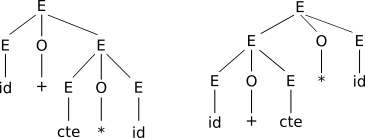
\includegraphics[width=0.6\textwidth]{img_18_1.png}
\caption{Arbol de derivación}\label{img_18_1}
\end{figure}
Luego $G$ es ambigua.

Para resolver esta ambigüedad que se debe a que no se ha definido un orden de prioridad entre los operadores , se considerará lo siguiente:
\begin{enumerate}
\item Los símbolos * y / tiene una prioridad más alta que + y -.
\item Si hay dos operaciones con igual prioridad realizar la evaluación de izquierda a derecha.
\end{enumerate}
Introducimos las variables:\\
T: término	\\
A: + ó -	\\
F: factor	\\
M: multiplicación y división	\\
Definimos las gramáticas equivalentes $G^2$.
\begin{align*}
&\Sigma_N=\{E,T,F,A,M\}\\
&S=E	\\
&E::=EAT|T	\\
&T::=TMF|F	\\
&F::=(E)|id|cte	\\
&A::=+|-	\\
&M::=*|div
\end{align*}
%GRAFICO2
\begin{figure}[h!]
\centering
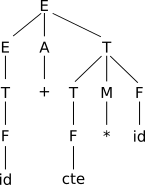
\includegraphics[width=0.3\textwidth]{img_18_2.png}
\caption{Arbol de derivación}\label{img_18_2}
\end{figure}

\section{Forma Normal de Greibach}
Una GLC está en la FNG si:
\begin{enumerate}
\item La variable inicial no es recursiva.
\item $G$ no tiene variables inútiles.
\item $G$ no tiene producciones $\varepsilon$( salvo $S\rightarrow\varepsilon$)
\item Todas las producciones son de la forma:
\begin{align*}
&A\rightarrow \sigma\qquad\mbox{(regla simple)}	\\
&A\rightarrow aB_1...B_k	\qquad\sigma,a\in\Sigma_T; B_i\in\Sigma_N	\\
\end{align*}
\end{enumerate}

\subsection{Características}
\begin{enumerate}
\item En cada paso de la derivación aparece un único símbolo terminal.
\item La derivación de una cadena de longitud $n$ $(n\geq 1)$ tiene exactamente $n$ pasos.
\end{enumerate}
\textbf{Método: }Para convertir una gramática a su FNG. realice estos pasos:
\begin{enumerate}
\item Enumere las variables en un orden arbitrario pero fijo en la que el símbolo $S$ sea la variable de orden.
\item Para cada variable de la gramática, $A$, de acuerdo al orden elegido, modifique las producciones de tal modo que el primer símbolo a la derecha de la flecha sea un terminal.
\item Utilice el \textbf{Lema} para modificar las variables originales de tal modo que el primer símbolo a la derecha de la flecha sea un terminal. Se debe seguir el orden inverso de enumeración de las variables: última, penúltima,etc.
\item Utilice de nuevo el \textbf{Lema}, para modificar las producciones de las variables nuevas, de tal modo que el primer símbolo a la derecha de la flecha sea un terminal.
\end{enumerate}

\textbf{Ejemplo: }Sea $G$ la GLC dada por:
\begin{align*}
&S::=AA|a	\\
&A::=AA|b
\end{align*}
Llevarla a su FNG
\textbf{Solución: }
\begin{enumerate}
\item El orden es S,A
\item Eliminamos la recursividad a la izquierda de la variable $A$. Introducimos la variable $Z$.
\begin{align*}
&A::=AA	\\
&A::=b	\\
&A::=b|bZ	\\
&Z::=A|AZ
\end{align*}
Luego, nos queda la gramática:
\begin{align*}
&S::=AA|a	\\
&A::=b|bZ	\qquad(*)	\\
&Z::=A|AZ
\end{align*}
Usamos(*) para reemplazar en las derivaciones de $S$
\begin{align*}
&S::=bA|bZA|a	\\
&A::=b|bZ	\\
&Z::=A|AZ
\end{align*}
Descomponemos las reglas de $Z$ por: 
\begin{align*}
&Z::=A	\\
&Z::=AZ	
\end{align*}
Usando $A::=b|bZ$, se obtiene finalmente:
\begin{align*}
&S::=bA|bZA|a	\\
&A::=b|bZ	\\
&Z::=b|bZ|bZZ
\end{align*}
Finalmente ya está en la FNG.
\end{enumerate}



\section{Automatas Push Down}

Arquitectura
%grafico por cambiar
\begin{figure}[h!]
\centering
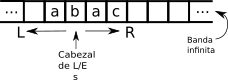
\includegraphics[width=0.3\textwidth]{img_19_1.png}
\caption{Máquina de Turing}\label{img_19_1}
\end{figure}

Un automata nde pila determinista (PDA-D) es una séptupla $$M=(S,\Sigma,s_0,\Gamma,\gamma_0,\delta,F)$$

\begin{tabular}{rl}
$S$			&	: Conjunto de estados	\\
$\Sigma$	&	: Alfabeto de la cinta	\\
$\Gamma$	&	: Alfabeto de pila	\\
$s_0$			&	: Estado inicial $s_0\in S$	\\
$\gamma_0$	&	: Simbolo en la cima de la pila\\
$\Delta$    & : Es la funcion de transicion. \\
$\Delta     & :S x (\Sigma U \{ \varepsilon \}) x\Gamma \rightarrow S x \Gamma^{*}$ \\
F			&	: Conjunto de estados de aceptación $(F\subseteq S)$	\\
\end{tabular}

\subsection{Paso computacional}

La transicion $\Delta(s_1,a,z) = (s_2,v)$ se le denominará un paso computacional.

Graficamente:

% dibujo




Casos especiales:

\begin{enumerate}
    \item $\Delta(s_1,a,z) = (s_2,z)$. El contenido de la pila no se altera.
    \item $\Delta(s_1,a,z)=(s_2,\varepsilon)$. Se borra el simbolo Z ubicado en la cima de la pila, y el control pasa a leer la nueva cima de la pila.
    \item $\Delta(s_1,\varepsilon,z)=(s_2,w)$
\end{enumerate}
Esta es una transicion $\varepsilon$. No se procesa el simbolo de la cinta de entrada, la unidad de control no se mueve a la derecha. En la cima reemplazamos Z por la cadena w.

Para garantizar el determinismo solo debe estar definido:
$$
\Delta (s,a,z) \mbox{ o } \Delta (s,\varepsilon,z);a\in\Sigma
$$

Configuracion instantanea

Es una terna de forma:
$$
(s,au,zv)
$$

Representa:
El automata esta en el estado s.
au es la parte no procesada de la cadena.
El cabezal apunta al simbolo a.
La cadena zv es el contenido total de la pila.

Para representar el paso computacional, escribiremos:
$$
(s_1,au,zw)\rightarrow (s_2,u,tw)
$$

El automata utilizo la transicion $\Delta (s_1,au,zw) = (s_2,t)$

La notación: $(s_1,u,\beta) \rightarrow^{*}(s_2,v,\gamma) $ significa el automata pasa de la CI $(s_1,u,\beta)$ a la CI $(s_2,v,\gamma)$ en cero, uno o mas pasos computacionales.

Configuracion inicial

Para una cadena $w \in \Sigma^{*}$, la configuración inicial es: $(s_0,w,\gamma)$.
El contenido inicial es $\gamma_0$ al iniciar el procesamiento de la cadena.

Configuracion de aceptación

La configuración $(s_a,\varepsilon,\beta)$ se llama de aceptacion si $s_a \in F$ y ademas se debe haber procesado toda la cadena. La cadena $\beta$ que queda en la pila puede ser cualquier cadena de simbolos en $\Gamma^{*}$


Lenguaje aceptado por una APD

Representa el lenguaje aceptado por un PDA-D mediante:
$$
L(P) = \{w\in \Sigma^{*}/(s_0,w,\gamma_0)\rightarrow^{*}(s_a,\varepsilon,\beta) \}
$$
Donde $s_0 \in S$, $s_a \in F$, $\beta \in \Gamma^{*}$

Teorema: Todo lenguaje regular L es aceptado por algun PDA-D

Prueba:

Sea $M_1=(S,\Sigma,\delta,s_0,F)$ un AFD que acepta a L.\\
El PDA-D $M_2 = (S,\Sigma,\Gamma,\Delta,s_0,\gamma_0,F)$ definido haciendo $\Gamma = \{\gamma_0\}$ y $\Delta (s,a,\gamma_0)=(\delta(s,a),\gamma_0)$  $\forall a\in \Sigma, \gamma_0 \in \gamma$ \\

Satisfacer $L(M_1) = L(M_2)$

Ejm: Diseñar un PDA-D M que acepte el lenguaje
$$
L = \{ a^i b^i / i \geq 1\} \mbox{ sobre } \Sigma=\{a,b\}
$$

Sol: Consideramos el PDA-D
$$
M = (S,\Sigma)
$$
...

La función de transicion $\Delta$ esta dada por:\\
\begin{tabular}{rl}
$\Delta(s_0,a,\gamma_0)$			&	$d$	\\
$\Sigma$	&	: Alfabeto de la cinta	\\
$\Gamma$	&	: Alfabeto de pila	\\
$s_0$			&	: Estado inicial $s_0\in S$	\\
$\gamma_0$	&	: Simbolo en la cima de la pila\\
$\Delta$    & : Es la funcion de transicion. \\
F			&	: Conjunto de estados de aceptación $(F\subseteq S)$	\\
\end{tabular}



